\documentclass[conference]{IEEEtran}
\usepackage{graphicx}
\usepackage{booktabs}
\usepackage{amsmath,amssymb}
\usepackage{url}

\title{Investigating Coordination Signals in Multi-Agent Tool-Using Language Models}

\author{\IEEEauthorblockN{Dhruva N}
\IEEEauthorblockA{Department of Artificial Intelligence and Machine Learning\\
Faculty of Engineering, PES University\\
Bengaluru, India}}

\begin{document}
\maketitle

\begin{abstract}
Task success alone does not reveal how language-model agents coordinate their actions. We compare single-agent, independent multi-agent, and coordination-oriented policies in a controlled synthetic tool-use task with matched fixture assignments. Each policy completed 64 episodes across 16 fixture variants, yielding 192 final episodes. Overall, 187 episodes succeeded, five were partial, and none failed. The observed success rates were 100.0\%, 93.75\%, and 98.44\%, respectively; reported paired fixture-cluster bootstrap intervals for all contrasts included zero. All five partial episodes ended in premature finalization on billing fixtures despite unused call budget. The environment logged 1,181 tool events, while a priority-compressed action-profile analysis yielded small exploratory mutual-information estimates. Because the policies differ in actor-assignment authority, the outcomes are near ceiling, and the profile encoding discards action order, these observations do not establish causal coordination or policy superiority. They show how constrained, auditable action traces can expose stopping behavior and support bounded descriptive comparisons.
\end{abstract}

\begin{IEEEkeywords}
large language models, multi-agent systems, coordination, tool use, synthetic evaluation
\end{IEEEkeywords}

\section{Introduction}

Multi-agent language-model evaluations often treat joint task completion as evidence of coordination. Yet a group can succeed without differentiated or mutually useful actions, and a group can exhibit structured behavior without improving the final outcome. Work on coordination and collective information motivates examining relations among actions and task state rather than relying on aggregate success alone \cite{riedl,agashe}.

Prior work examines reasoning and action in language models, tool-use benchmarks, and configurable multi-agent frameworks \cite{yao,api,camel,autogen}. We study three sequential tool-use policies---single-agent, independent multi-agent, and prompted coordination---in a synthetic software-repair environment. The experiment is designed to make action selection and terminal state observable, not to model unrestricted code repair. The research questions are descriptive: how do matched episode outcomes differ, how do tool use and actor attribution vary, and when do policies finalize with unresolved work?

\section{Methods}

The environment contains eight fixture families and 16 variants. Each provides declared defects, exact catalog patches, state-filtered valid actions, and synthetic checks. Policies select among five tools: retrieve a file, search a symbol, apply a patch, run fixture checks, or finalize. The evaluator classifies each episode as success, partial, or failure; its checks do not execute modified source code. A valid patch changes simulated fixture state. Accordingly, tool validity and patch acceptance describe interaction with the constrained environment, not correctness of a generated repair in a real repository.

Each episode has a 12-call budget. At each decision, the model receives current shared task state, the last six selected actions, actor identifiers, and the current valid-action list, and must return one matching tool-and-arguments selection. Decisions occur sequentially against one shared environment; the adapters do not provide concurrent agent calls, direct peer messaging, separate observations, or persistent private agent memory. The single-agent adapter attributes actions to actor 0. The independent adapter schedules actors in alternating order, while the prompted-coordination adapter allows the model to assign an action to either nominal actor. Both multi-agent conditions use a shared policy-level history. The coordinator therefore changes both the role instruction and authority over actor assignment, so the conditions do not isolate a prompt-only effect.

The matched design crosses all three policies with the same 16 variants and four repetitions per variant, using explicit fixture, repetition, and seed identities. The resulting 192 final episodes are one completed trace per manifest identity. Collection failures and task outcomes have separate denominators: the first pass completed 169/192 identities; 23 initially failed identities later completed after 56 failed whole-episode attempts, giving 248 executions in total. An invalid model response can trigger a response-level retry before an accepted action is applied; such responses are not environment-invalid calls. The strict audit records these recovery events separately from final episode summaries.

We report outcome counts and percentages, calls per completed episode, tool totals, and actor-attributed traces. Paired outcome contrasts use the report's 10,000-resample fixture-variant cluster bootstrap. For exploratory analysis, each actor's complete event history is compressed to its highest-priority action category; the ordered pair is compared with binary outcome using plug-in mutual information. The report's outcome-label permutations and episode-bootstrap intervals are within-policy diagnostics: they neither adjust for fixture family nor compare policies' MI values. Because the source report does not provide independently regenerated episode-level counts here, the inferential interval values below are reproduced as reported.

\section{Results}

There were 187 successes (97.4\%), five partial outcomes, and no failures. Success counts were 64/64 for single-agent, 60/64 for independent multi-agent, and 63/64 for prompted coordination. Paired success-rate differences were +6.25, +1.56, and +4.69 percentage points for single-agent minus independent, single-agent minus prompted, and prompted minus independent, respectively. The reported 95\% fixture-cluster bootstrap intervals were [0.00, 15.62], [0.00, 4.69], and [0.00, 12.50] points; each includes zero.

\begin{table}[t]
\caption{Outcome and event-count summary by policy.}
\label{tab:policy-results}
\centering
\footnotesize
\begin{tabular}{lrrrr}
\toprule
Policy & Success & Partial & Calls & Calls/episode\\
\midrule
Single-agent & 64/64 & 0 & 416 & 6.50\\
Independent multi-agent & 60/64 & 4 & 394 & 6.16\\
Prompted coordination & 63/64 & 1 & 371 & 5.80\\
\bottomrule
\end{tabular}
\end{table}

\begin{figure}[t]
\centering
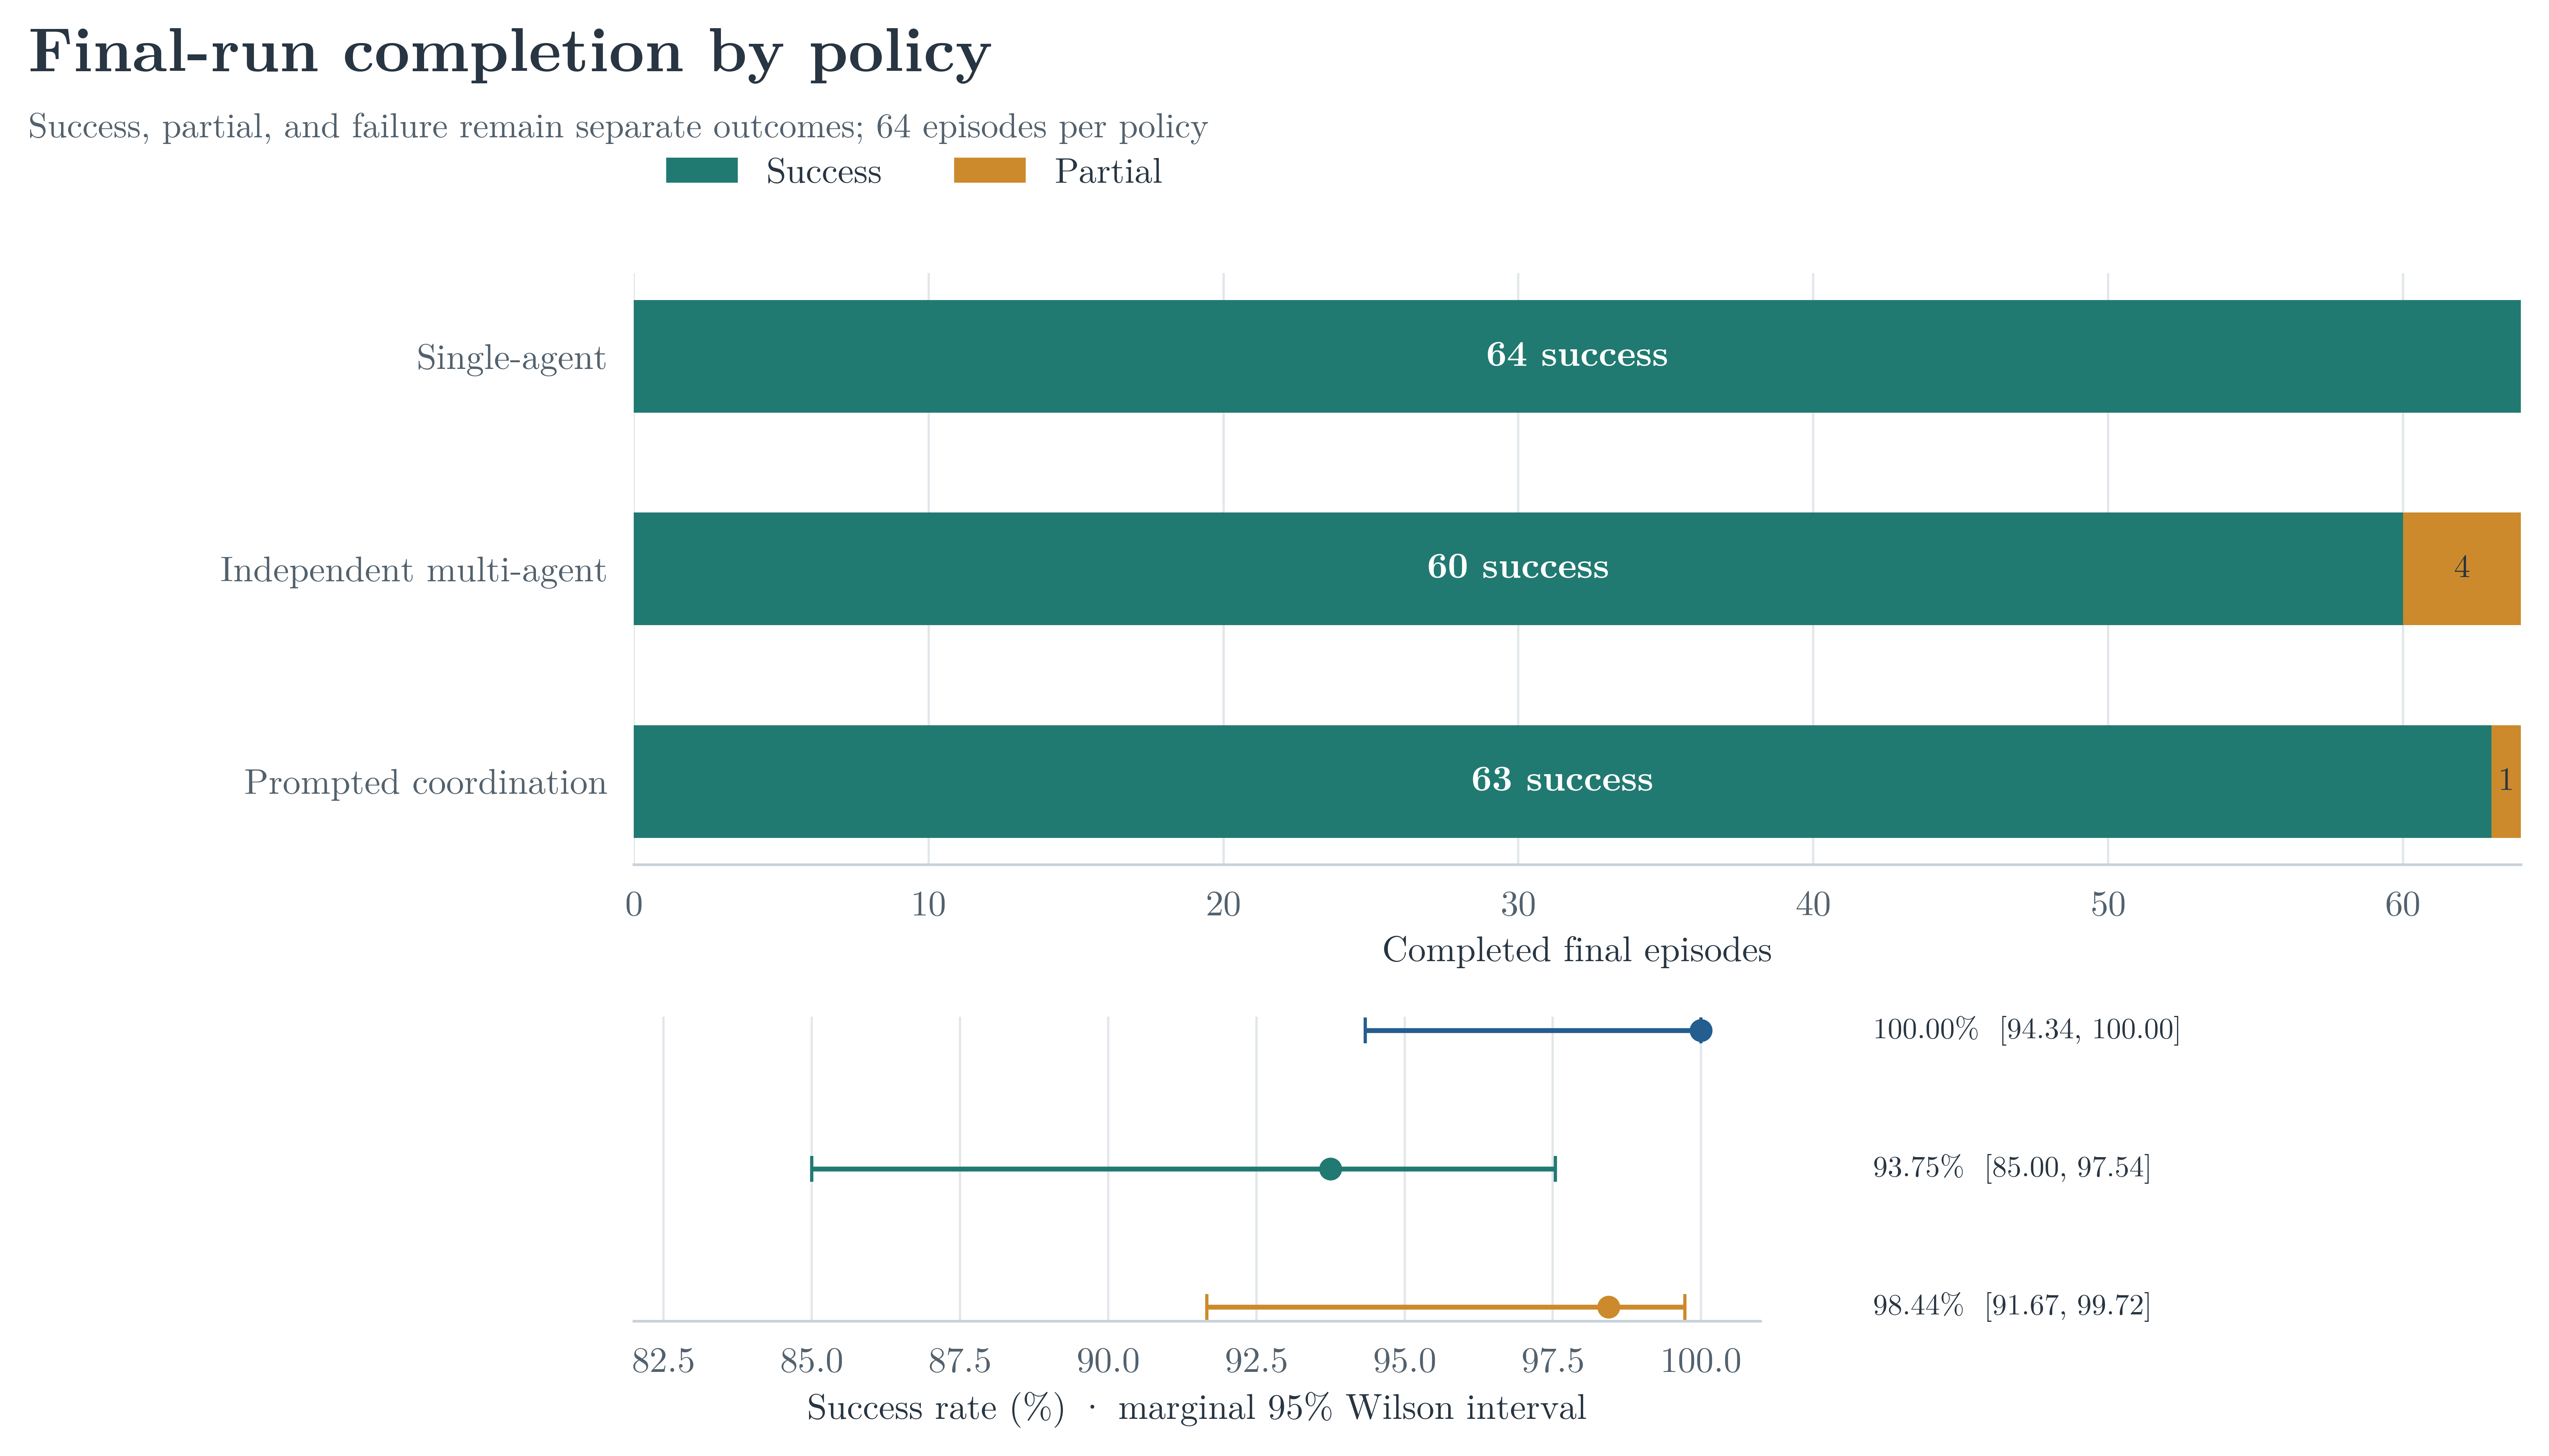
\includegraphics[width=\columnwidth]{../Project_report/Images/09_final_outcomes.png}
\caption{Final outcomes by policy; marginal Wilson intervals are not paired policy tests.}
\label{fig:outcomes}
\end{figure}

All five partials were billing episodes finalized after four to six calls, with required work incomplete and budget remaining. The two discount-order partials (both independent multi-agent) left the primary defect unresolved after five and six calls. Two independent and one prompted-coordination invoice-total episodes left the tertiary defect unresolved after five, five, and four calls, respectively. The single-agent policy completed the matched billing assignments successfully. The immediate recorded stopping behavior was early finalization, not exhaustion of the 12-call budget; the traces do not establish why the model finalized.

The 1,181 final-trace events comprised 175 file-retrieval calls, 65 symbol searches, 403 patch calls, 346 test calls, and 192 finalizations. All 403 supplied patch actions were accepted, and no submitted environment call was invalid. These rates reflect a dynamically filtered allow-list containing exact catalog patches, rather than unrestricted code generation. A \texttt{run tests} action evaluates fixture-declared state and checks; it does not run tests against the changed code. The prompted condition used the fewest calls on average, but fewer calls are not evidence of greater efficiency when completion and unresolved work differ.

The strict response audit recorded 96 recoverable invalid model responses across 81 episodes. At the separate collection level, 56 failed whole-episode attempts preceded completion of all 192 identities. The independent condition had 11 first-pass failures, compared with seven for single-agent and five for prompted coordination; every affected identity was eventually completed. These counts are operational reliability observations, not task failure counts. Since response failure may be related to policy or fixture behavior, the eventual completed-trace outcomes should not be mistaken for a uniformly capped first-pass evaluation.

Action-profile mutual information was 0.0466 bits for independent multi-agent ($n=64$, 95\% bootstrap interval [0.0017, 0.1976], permutation $p=0.207$) and 0.0400 bits for prompted coordination ($n=58$, interval [0.0000, 0.1258], $p=0.386$). The coordinator's paired estimate excludes six episodes in which only one nominal actor had any recorded event. Retaining all 64 with a \texttt{no actions} category gives a reported point estimate of 0.0385 bits, without an interval or permutation test. The profiles retain only each actor's highest-priority category, discarding order and earlier work; every paired profile contains a finalization category. All five partials also come from billing, so fixture composition may influence both the profile and outcome. These sparse estimates are exploratory associations, not validated coordination scores.

\section{Discussion and conclusion}

Explicit state-linked actions made it possible to identify premature finalization as the immediate recorded behavior in every partial episode. The concentration of partial outcomes in billing also shows why pooled completion rates can hide a localized difficulty in this engineered catalog. These observations motivate measuring stopping quality, retaining action sequences, and evaluating a broader range of task difficulty.

Interpretation of tool and actor counts depends on how actions are generated. State-filtered prompts include exact recognized patch replacements, while fixture tests do not execute patched code. Perfect environment acceptance thus reflects compliance with supplied options. Similarly, independent alternation and model-selected actor attribution are not equivalent opportunities for specialization: the latter can change pooled workload by design. Neither acceptance rates nor actor imbalance demonstrates that the model discovered a useful role division.

This study is bounded to one model/provider configuration, one engineered fixture catalog, and three policy implementations. The small, near-ceiling outcome differences do not establish superiority, causal coordination, or emergent specialization. Fixture-matched assignments support comparisons within the catalog but do not make the eight task families a random sample of real repair work. The mutual-information analysis is especially limited by sparse outcomes, lossy categories, and fixture-level confounding. The defensible conclusion is that auditable tool traces support descriptive comparisons in this synthetic setting; stronger claims require separated policy interventions, broader validated tasks, independently executed repairs, and trajectory measures that preserve action order.

\begin{thebibliography}{6}
\bibitem{riedl} C. Riedl, ``Emergent Coordination in Multi-Agent Language Models,'' arXiv:2510.05174v4, 2026.
\bibitem{agashe} S. Agashe, Y. Fan, A. Reyna, and X. E. Wang, ``LLM-Coordination: Evaluating and Analyzing Multi-agent Coordination Abilities in Large Language Models,'' arXiv:2310.03903, 2023.
\bibitem{yao} S. Yao et al., ``ReAct: Synergizing Reasoning and Acting in Language Models,'' in Proc. International Conference on Learning Representations, 2023.
\bibitem{api} M. Li et al., ``API-Bank: A Comprehensive Benchmark for Tool-Augmented LLMs,'' arXiv:2304.08244, 2023.
\bibitem{camel} G. Li et al., ``CAMEL: Communicative Agents for `Mind' Exploration of Large Language Model Society,'' in Advances in Neural Information Processing Systems, vol. 36, 2023.
\bibitem{autogen} Q. Wu et al., ``AutoGen: Enabling Next-Gen LLM Applications via Multi-Agent Conversation,'' arXiv:2308.08155, 2023.
\end{thebibliography}

\end{document}
